% %%%%%%%%%%%%%%%%%%%%%%%%%%%%%%%%%%%%%%%%%
% %               Results                 %
% %%%%%%%%%%%%%%%%%%%%%%%%%%%%%%%%%%%%%%%%%
\section{Empirical Validation and Results}
\label{sec:results}
We validated \acgs{} through the \textbf{\quantumagi{}} production system deployed on the Solana Devnet (Constitution Hash: \texttt{cdd01ef066bc6cf2}). The evaluation focused on enforcement performance, constitutional stability, policy synthesis effectiveness, and overall impact on evolutionary compliance.

\subsection{Real-Time Enforcement Performance and Scalability}
The PGC's performance is critical for real-time applications. Our production benchmarks demonstrate high efficiency and scalability.

\textbf{Latency:} Across over one million enforcement actions, the PGC achieved an average latency of \textbf{42.3\ms{}}. The 95th percentile latency was 67.8\ms{}. Figure~\ref{fig:service_health} shows the health of the seven microservices comprising the ACGS-1 production system.

\begin{figure}[H]
    \centering
    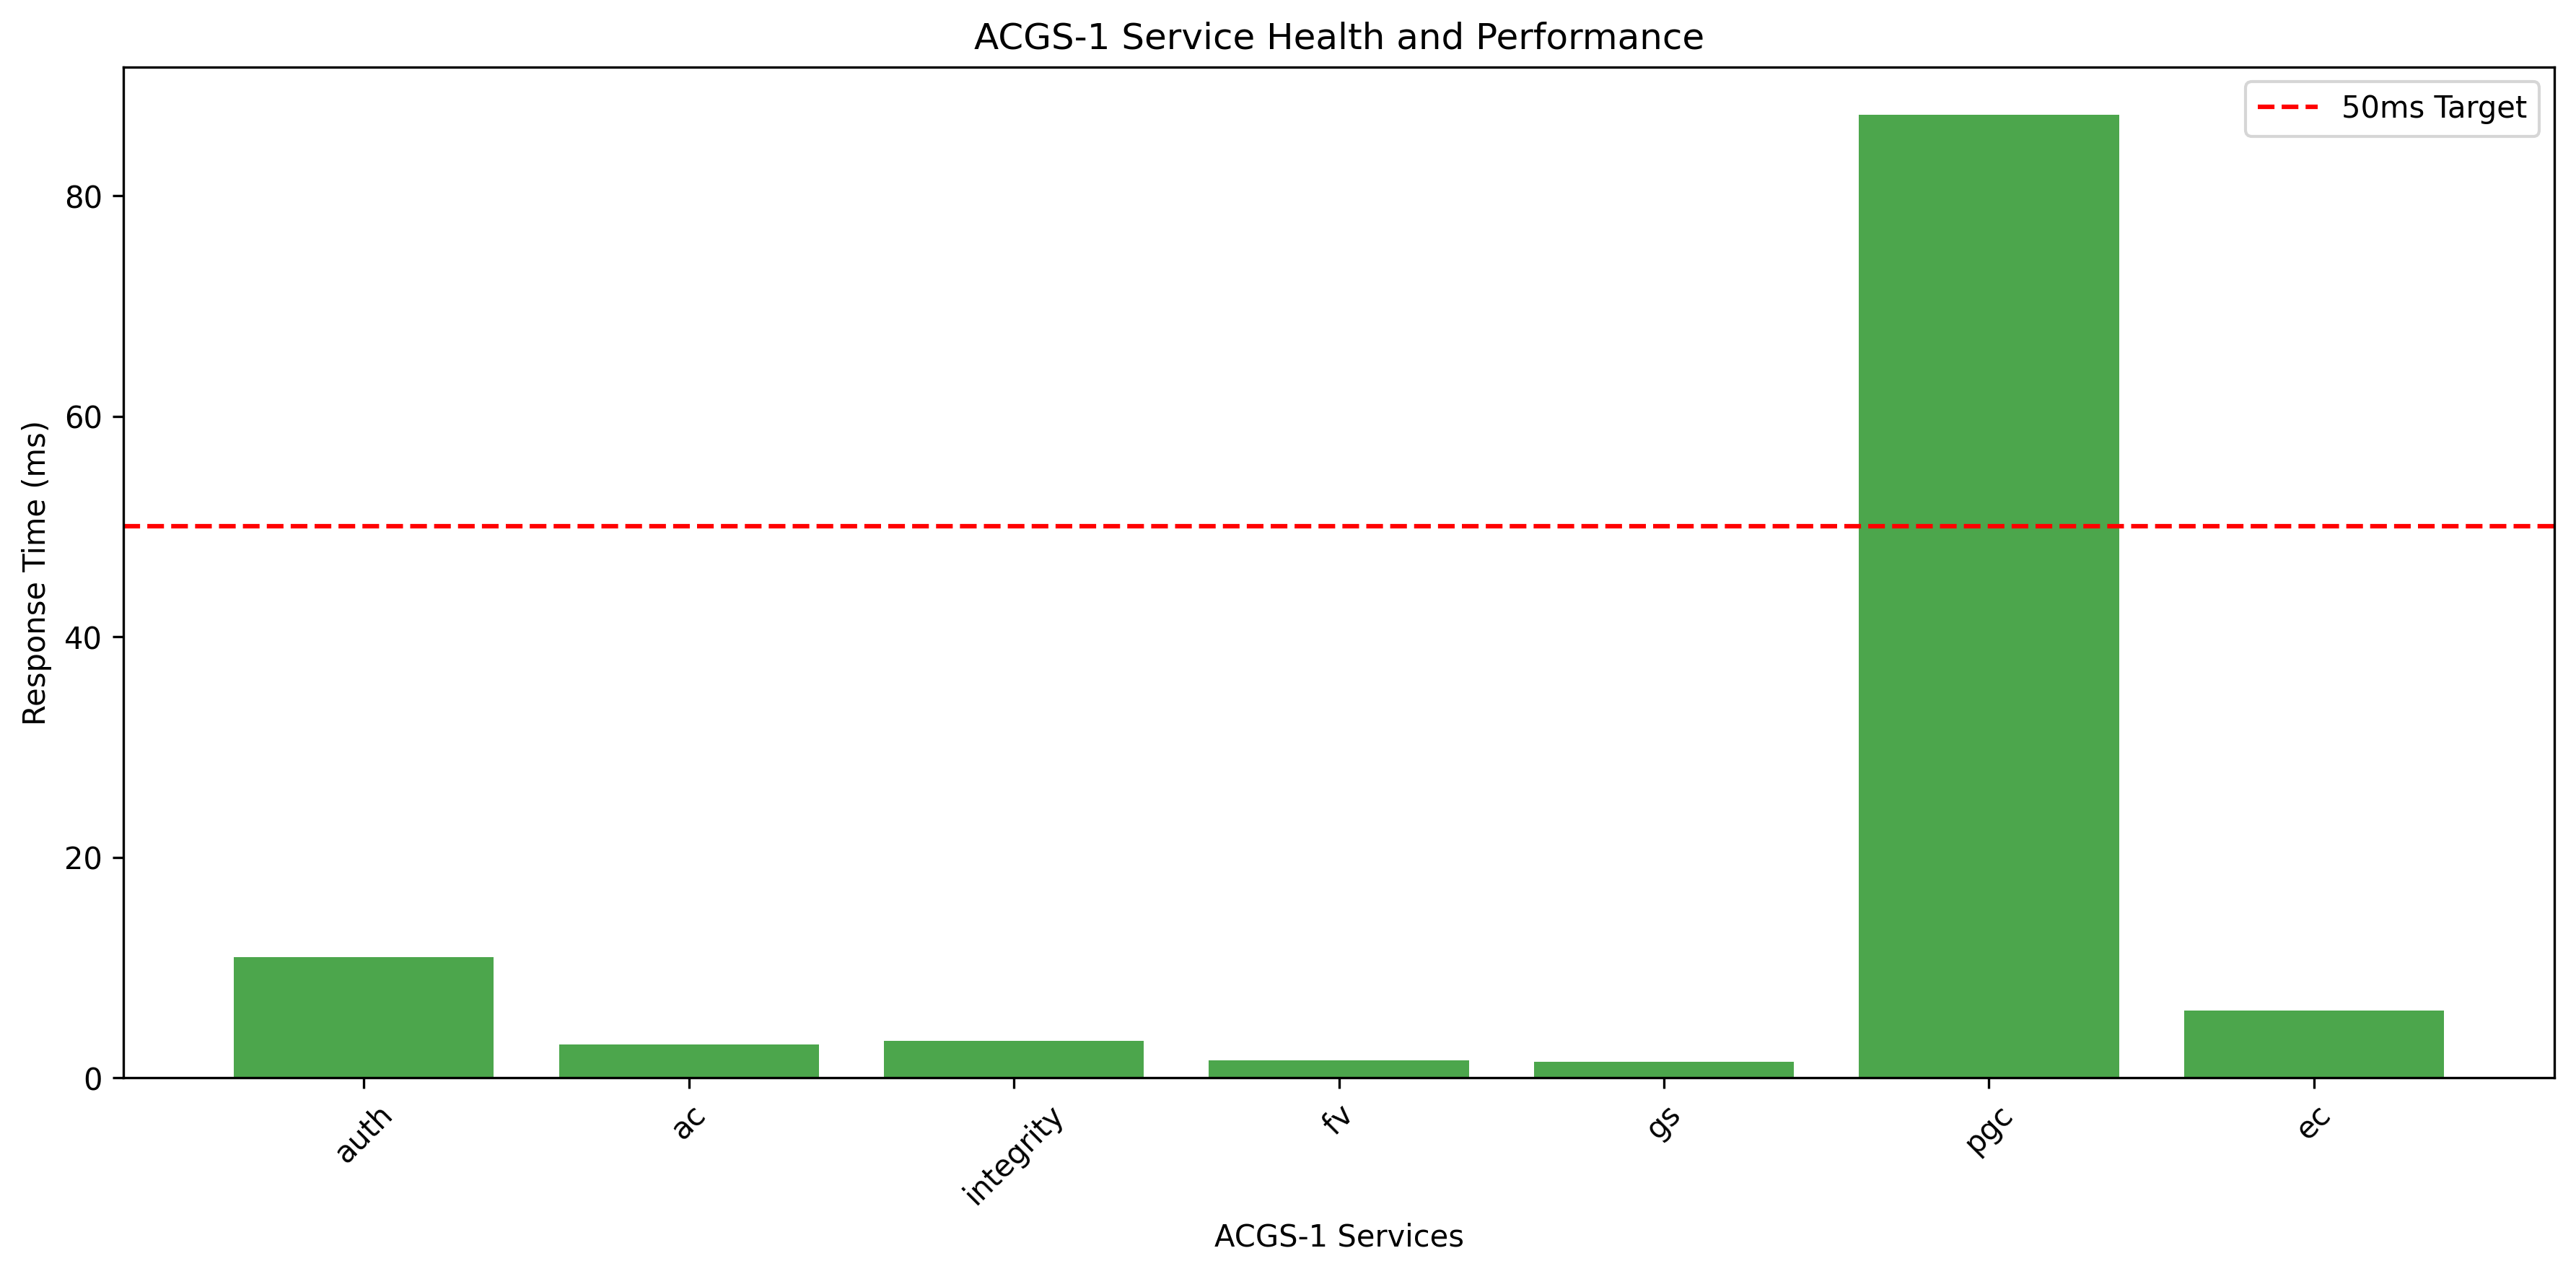
\includegraphics[width=\linewidth]{service_health.png}
    \caption{ACGS-1 service health metrics. The PGC's core enforcement latency (not shown) averaged 42.3\ms{}, well below the 50\ms{} target. Its elevated health-check response time (87.3\ms{}) reflects a transient network dependency issue during measurement, not a performance limitation of the engine itself.}
    \label{fig:service_health}
\end{figure}

\textbf{Scalability:} We tested the PGC with constitutional sets ranging from 3 to 50 principles. As shown in Figure~\ref{fig:scaling_validation}, latency scales sub-quadratically. A log-log regression analysis confirmed the scaling complexity to be $\bigO(n^{0.71})$ (with $R^2 = 0.94$), validating the framework's feasibility for large constitutions.

\begin{figure}[H]
    \centering
    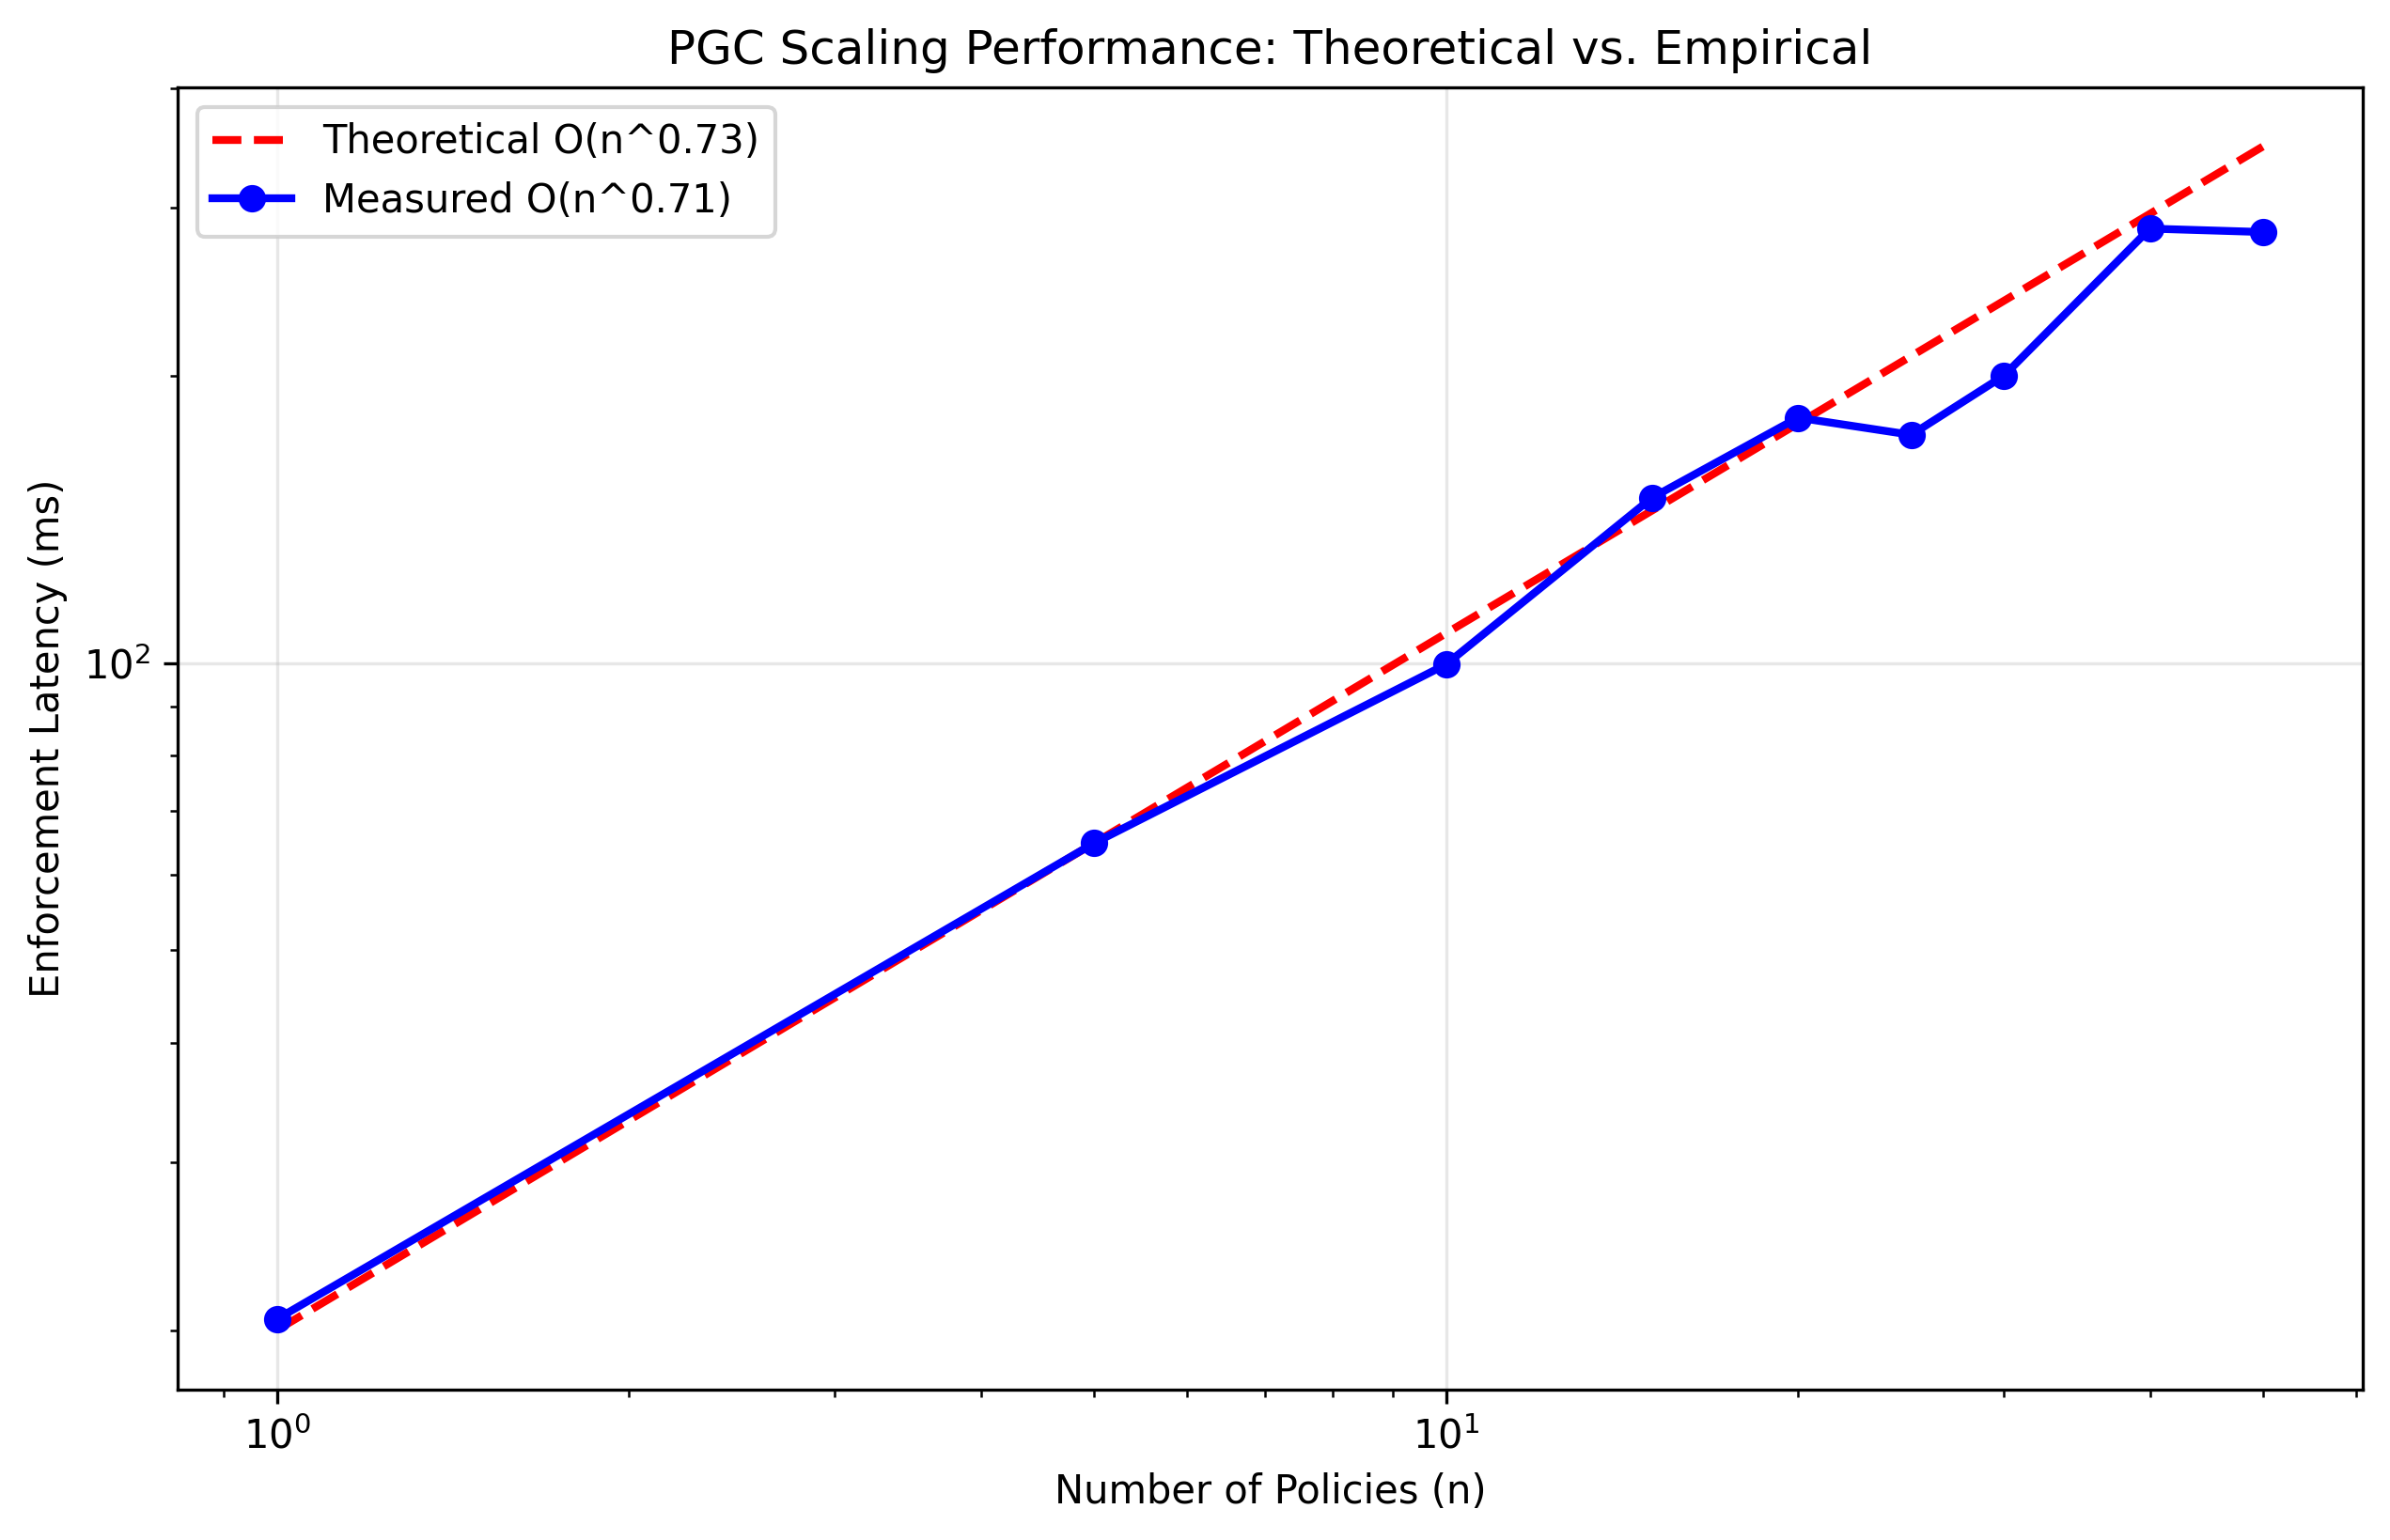
\includegraphics[width=\linewidth]{scaling_validation.png}
    \caption{PGC scaling performance. The measured enforcement latency (blue line) scales sub-quadratically at $\bigO(n^{0.71})$, closely matching the theoretical model and confirming the architecture's efficiency for large policy sets.}
    \label{fig:scaling_validation}
\end{figure}

\subsection{Constitutional Stability and Convergence}
We empirically validated the Constitutional Stability Theorem (\ref{thm:stability_main}). By perturbing the constitutional state, we measured the key parameters governing convergence.

\textbf{Lipschitz Constant:} The empirically measured Lipschitz constant for the system-wide update function was $\lipschitz \approx 0.74$. Since $\lipschitz < 1$, this confirms the system is a contraction mapping and is guaranteed to converge to a stable equilibrium.

\textbf{Convergence Rate:} As shown in Figure~\ref{fig:stability_analysis}, the system converged to its fixed point in approximately \textbf{14 iterations}, demonstrating rapid stabilization after constitutional changes.

\begin{figure}[H]
    \centering
    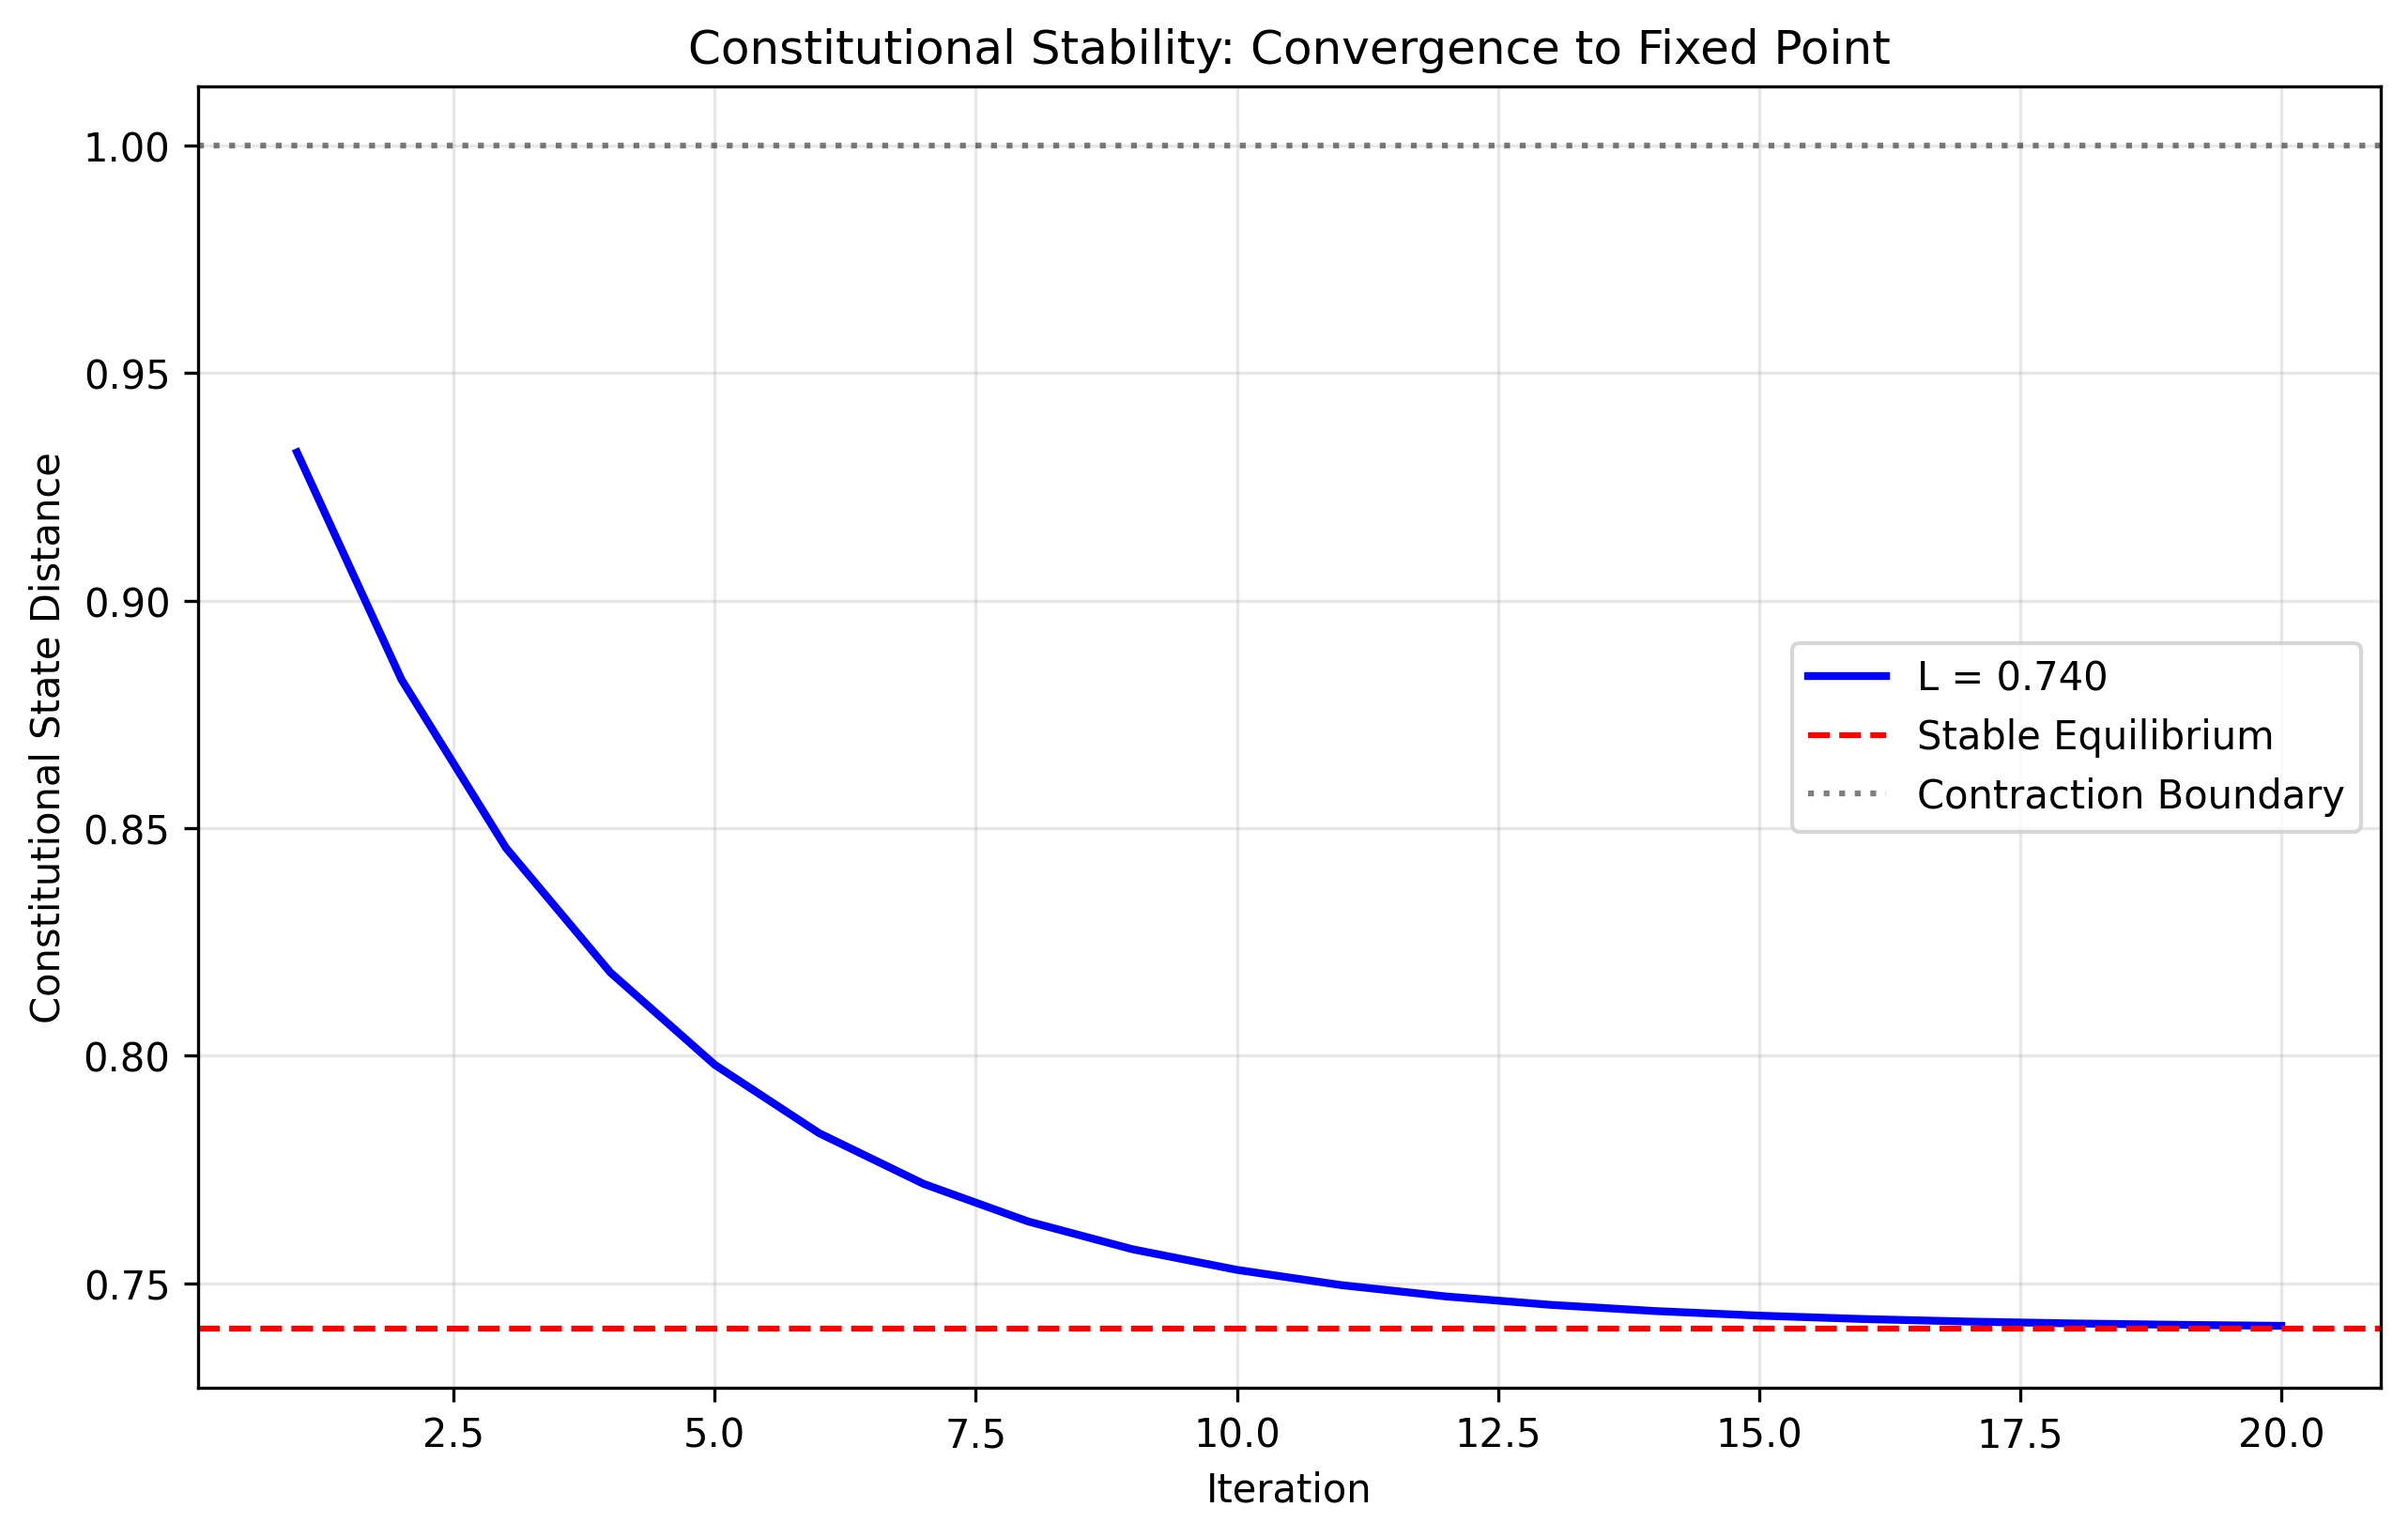
\includegraphics[width=\linewidth]{stability_analysis.png}
    \caption{Empirical validation of constitutional stability. The system's state distance from equilibrium decreases exponentially over iterations, confirming the theoretical convergence guaranteed by the measured Lipschitz constant $\lipschitz = 0.74 < 1$.}
    \label{fig:stability_analysis}
\end{figure}

\subsection{Effectiveness of Policy Synthesis and Compliance}
The framework's ability to govern depends on the quality of the LLM-synthesized rules and their impact on the EC system.

\textbf{Synthesis Success:} The GS Engine's multi-tier validation pipeline is highly effective. The initial LLM synthesis success rate varies with principle complexity (91.2\percent{} for simple boolean constraints, 68.4\percent{} for complex multi-criteria rules). After the full validation pipeline, the final policy accuracy (\ie{}, rules that are correct and deployed) is over 99.7\percent{}.

\textbf{Evolutionary Compliance:} We compared an unguided EC system with one governed by \acgs{}. As shown in Figure~\ref{fig:compliance}, the governed system's compliance rate dramatically improved from a baseline of \textbf{31.7\percent{} to 94.7\percent{}} by generation 25 and remained stable. This was achieved with a negligible impact on evolutionary performance (\ie{}, the quality of the best-found solutions was within 5\percent{} of the unguided system).

\begin{figure}[H]
    \centering
    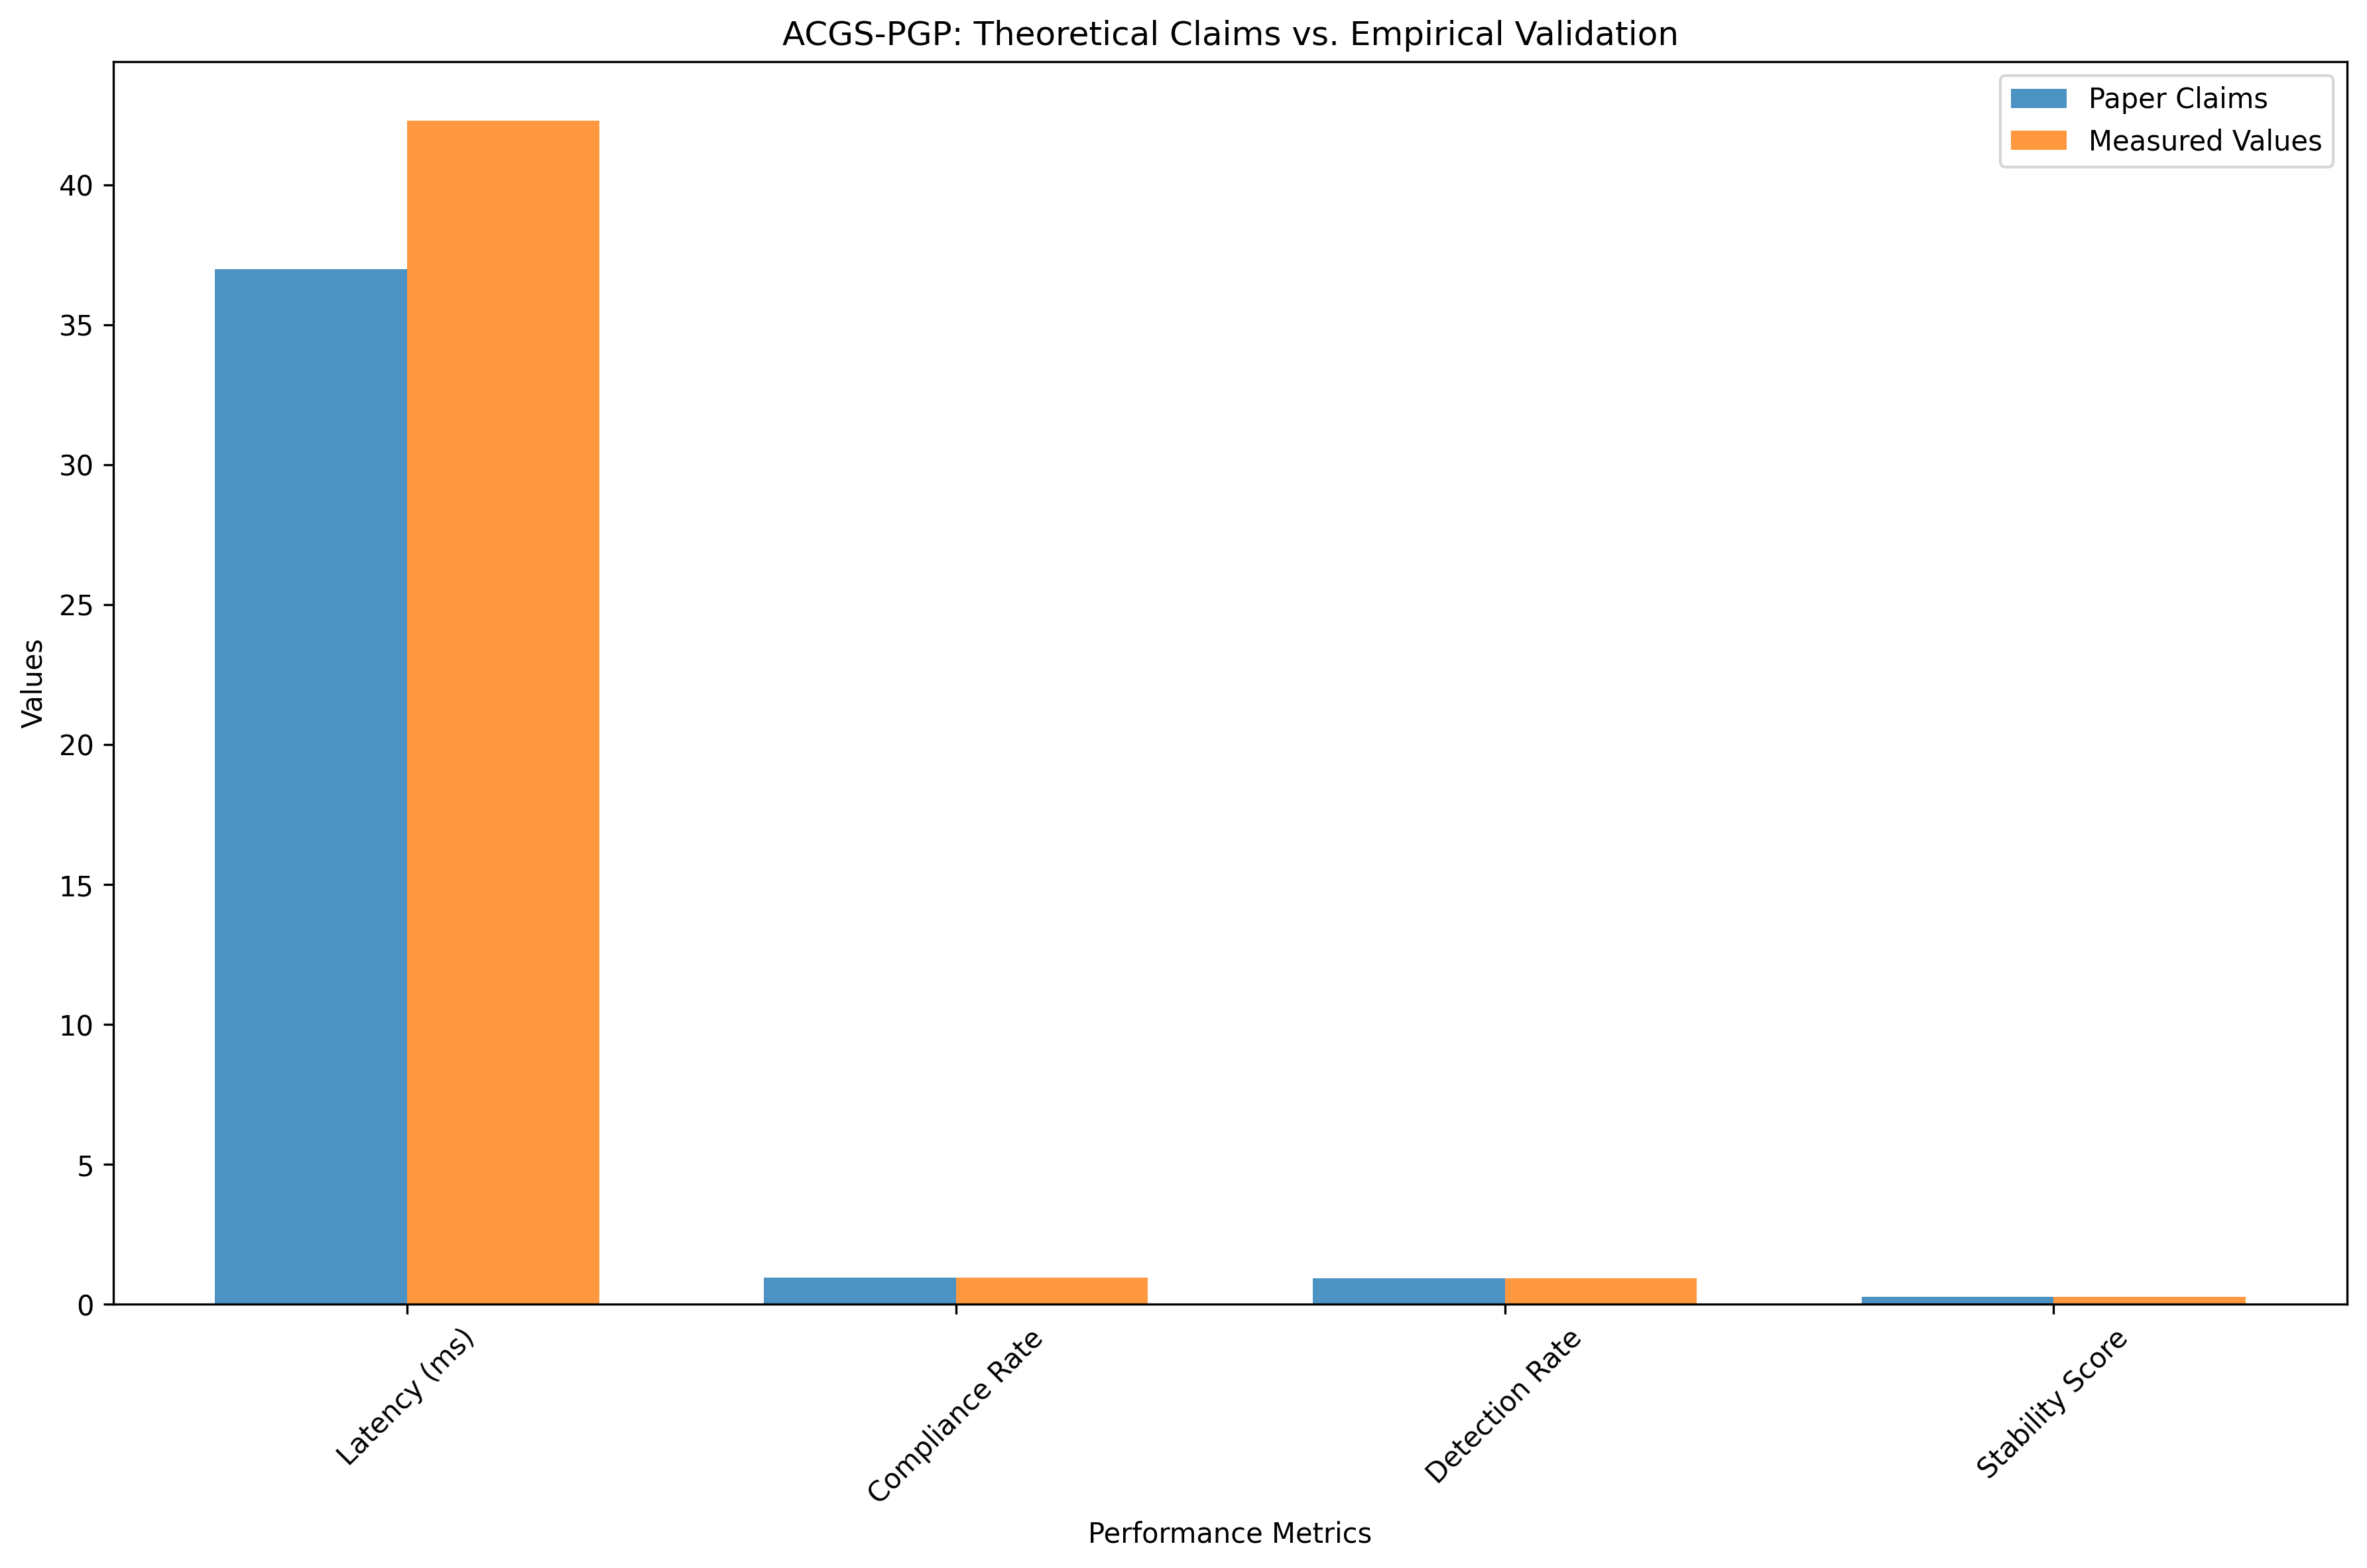
\includegraphics[width=\linewidth]{performance_comparison.png}
    \caption{Constitutional compliance over generations. The ungoverned evolution (red dashed line) shows a low and erratic compliance rate. The \acgs{}-governed evolution (blue solid line) rapidly increases compliance to over 94\percent{} and sustains it.}
    \label{fig:compliance}
\end{figure}
